\section{Linear Classification}

\subsection{Linear Classifier}

设有数据集 $\{(x_i,y_i)\mid i=1,2,\ldots,N\}$，其中 $x_i\in\mathbb R^D,\,y_i\in\{1,\ldots,K\}$.
定义 score function: $f:\mathbb R^D\mapsto \mathbb R^K$，即输入一个由图片像素构成的 $D$ 维向量，输出这个图片属于各个类别的 score. 我们认为 score 越高，图片越可能属于这个类别。

对于 linear classifier 来说，它的 score function 为：
\[
f(x;W,b)=Wx+b
\]
其中，$W\in\mathbb R^{K\times D},\,b\in\mathbb R^K$ 是参数，分别称作 weights 和 bias. 由于第 $i$ 类的得分为 $W$ 的第 $i$ 行与 $x$ 的内积加上 $b$ 的第 $i$ 个元素，因此类别之间的得分相互独立，写成矩阵只是为了方便而已。

为直观理解 linear classifier，注意到 $z=wx+b$ 是一个 $\mathbb R^{D+1}$ 中的超平面，法向量为 $(w,-1)$，截距为 $b$. 输入的 $x$ 在超平面上对应位置的“高度”越高，就越可能属于这一超平面代表的那一类。下面是 $D=2$ 的一个例子，线条表示超平面与 $z=0$ 的交线，沿着箭头方向走，$wx+b$ 变大。

\begin{figure}[H]
    \centering
    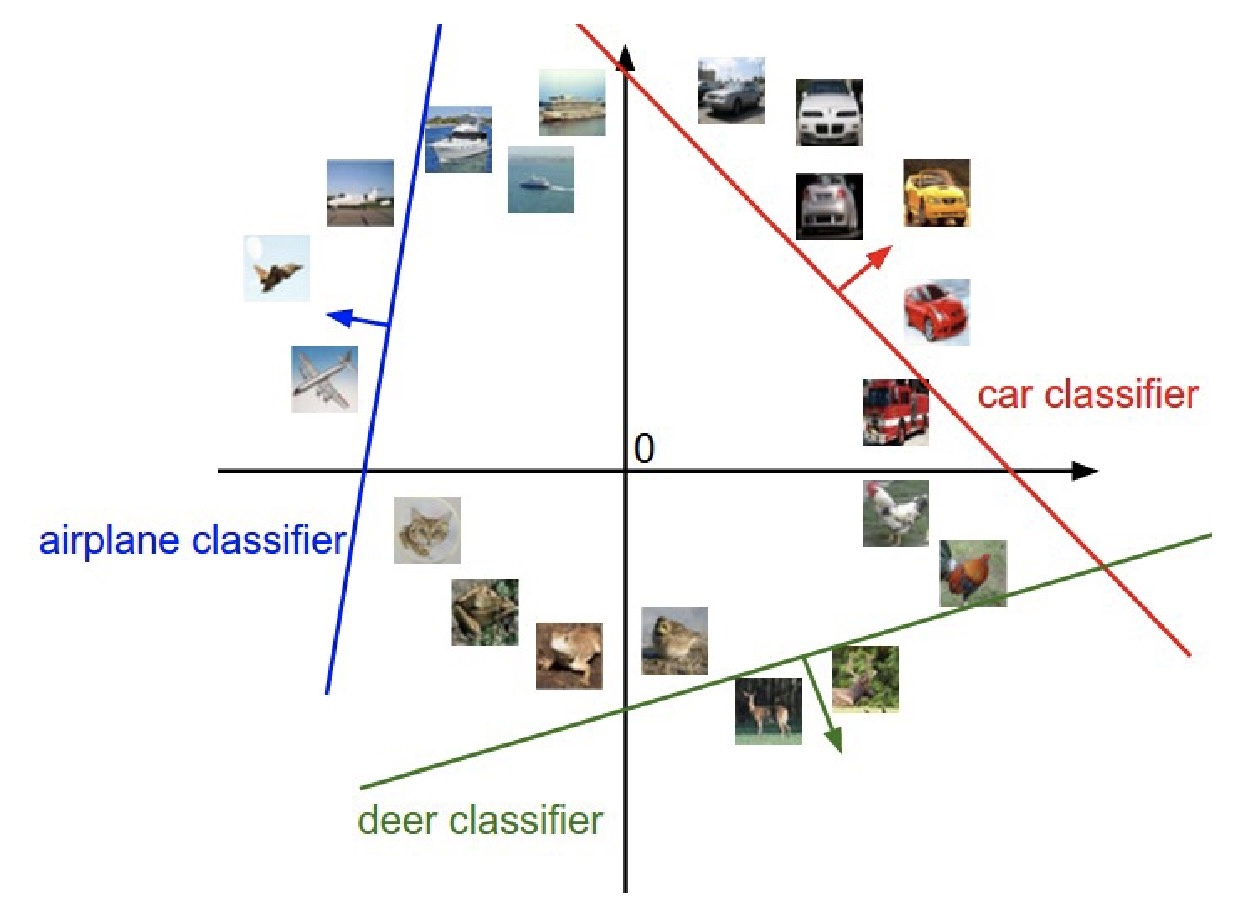
\includegraphics[width=0.5\linewidth]{figs/chapter2/linear classifier.jpg}
\end{figure}

为了获得参数 $W,b$，我们需要定义损失函数 (loss function)。训练 $W,b$ 就是最小化损失函数的过程，机器学习问题最终归结为一个优化问题。

\subsection{Multiclass SVM}

Multiclass SVM 是一种常用的损失函数. 对于数据 $(x_i,y_i)$，其损失定义为：
\[
L_i=\sum_{j\neq y_i}\max(0,s_j-s_{y_i}+\Delta)
\]
其中，$s_j$ 表示 $x_i$ 在第 $j$ 类上的得分，即 $s_j=f(x_i;W,b)_j$.

对这个损失函数的理解是，如果正确分类的得分 $s_{y_j}$ 比错误分类的得分 $s_j$ 还高一个 $\Delta$，那么损失就是 $0$；否则，损失是 $s_j+\Delta$ 比 $s_{y_j}$ 多出的部分。由于这个函数的图像形状像铰链（合叶），所以这种损失函数也称作 \textbf{hinge loss}.

在机器学习课程中我们学过正则化。若使用 L2 regularization，则 Multiclass SVM 的完整形式是：
\[
L=\frac{1}{N}\sum_{i=1}^N\sum_{j\neq y_i}\max(0,f(x_i;W,b)_j-f(x_i;W,b)_{y_i}+\Delta)+\lambda\sum_k\sum_lW_{kl}^2
\]
值得注意的是，上式中的 $\Delta$ 并不是需要调节的超参数，取 $\Delta=1$ 即可。这是因为 $W$ 的整体放缩可以在不改变 $s_j$ 和 $s_{y_i}$ 的大小关系的条件下改变它们的差值，所以 $\Delta$ 取值并不影响结果。

\subsection{Softmax classifier}

Softmax classifier 是二元逻辑回归分类器在多分类上的扩展，不同于 multiclass SVM，softmax classifier 的输出有一个概率的解释。
具体而言，对于数据 $(x_i,y_i)$，设 $f_j$ 表示它在第 $j$ 类上的得分，softmax classifier 视之为尚未标准化的对数概率，并采取 \textbf{cross-entropy loss} 作为损失函数：
\[
L_i=-\log\left(\frac{e^{f_{y_i}}}{\sum_j e^{f_j}}\right)
\]
其中，函数 $f_j(z)={e^{z_j}}/{\sum_ke^{z_k}}$ 称作 \textbf{softmax function}.

同样的，总的损失函数定义为各 $L_i$ 的平均值加上正则化项：
\[
L=-\frac{1}{N}\sum_{i=1}^N\log\left(\frac{e^{f_{y_i}}}{\sum_j e^{f_j}}\right)+\lambda\sum_k\sum_lW_{kl}^2
\]

从信息论角度理解，设真实概率分布为 $p$，估计概率分布为 $q$，则 cross-entropy 定义为：
\[
H(p,q)=-\sum_x p(x)\log q(x)
\]
在图像分类问题中，我们估计的各个分类上的概率分布为 $q=e^{f_{y_i}}/\sum_je^{f_j}$，而真实分布为 $p=[0,\ldots,1,\ldots,0]$（即正确的分类为 $1$，其余为 $0$ ）。Softmax classifier 最小化的就是 $H(p,q)$.

从概率论角度理解，
\[
\mathbb P(y_i\vert x_i;W)=\frac{e^{f_{y_i}}}{\sum_j e^{f_j}}
\]
可以解释为当参数为 $W,b$ 时，$x_i$ 的类别为 $y_i$ 的概率，因此最小化 $L_i$ 等价于实施极大似然估计。

值得注意的是，在编写代码时，$e^{f_j}$ 可能太大以至于计算精度较低，但是注意到：
\[
\frac{e^{f_{y_i}}}{\sum_j e^{f_j}}=\frac{Ce^{f_{y_i}}}{C\sum_j e^{f_j}}=\frac{e^{f_{y_i}+\ln C}}{\sum_j e^{f_j+\ln C}}
\]
所以我们可以取 $\ln C=-\max\limits_j f_j$ 来解决这个问题。

\subsection{SVM vs. Softmax}

\begin{figure}[H]
    \centering
    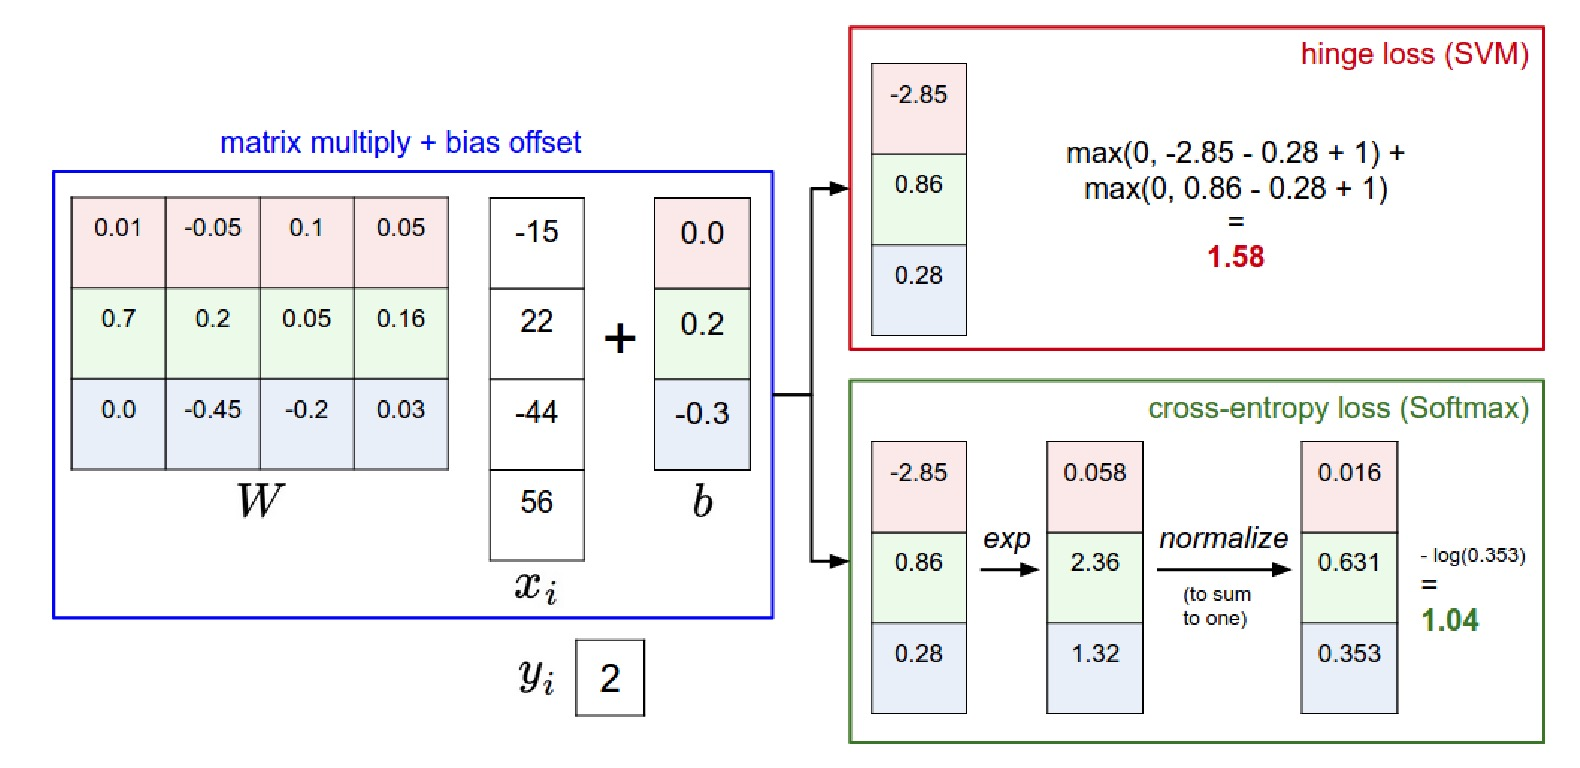
\includegraphics[width=0.8\linewidth]{figs/chapter2/svm vs softmax.jpg}
\end{figure}
